\documentclass[12pt]{standalone}

\usepackage{tikz}
\usepackage{ctex}

\usetikzlibrary{graphs}

\begin{document}
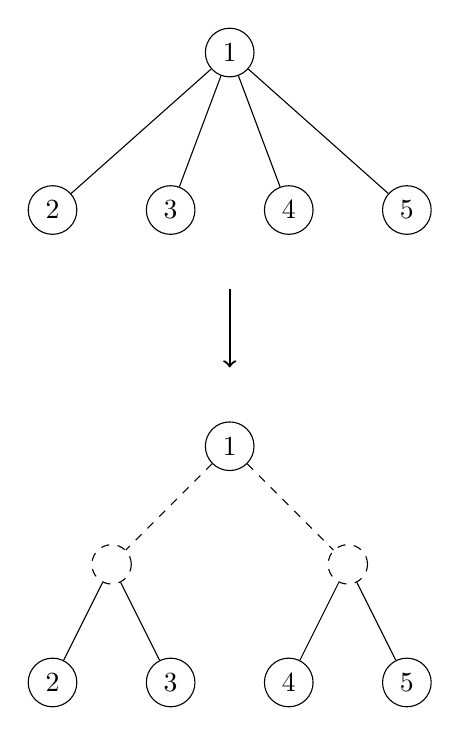
\begin{tikzpicture}[every node/.style={circle,draw,minimum size=5mm}]

\scoped[level distance=2cm]
\node at (0,0) {1}
    child {node {2}}
    child {node {3}}
    child {node {4}}
    child {node {5}};

\draw[->,thick] (0,-3) -- (0,-4);

\scoped[level 1/.style={sibling distance=30mm},
    level 2/.style={sibling distance=15mm}]
\node at (0,-5) {1}
    child[dashed] {node {}
        child[solid] {node {2}}
        child[solid] {node {3}}}
    child[dashed] {node {}
        child[solid] {node {4}}
        child[solid] {node {5}}};

\end{tikzpicture}
\end{document}
